 %	Main Document

\documentclass[
	12pt,
	BCOR=5mm,
	DIV=12,
	headinclude=on,
	footinclude=off,
	parskip=half,
	bibliography=totoc,
	listof=entryprefix,
	toc=listof,
	pointlessnumbers,
	plainfootsepline]{scrreprt}

% include configuration file
% !TEX root =  master.tex

% language, font, colors
\usepackage[ngerman]{babel}
\usepackage[utf8]{inputenc}
\usepackage[german=quotes]{csquotes} 	% correct quotes using \enquote{}
\usepackage[T1]{fontenc}
\usepackage{lmodern} % latin modern font, TODO: Arial 12?
\usepackage[onehalfspacing]{setspace}
\usepackage{xcolor}

% hyperlinks
\usepackage[hidelinks=true]{hyperref}

% commands for author and title
\newcommand{\TitelDerArbeit}[1]{\def\DerTitelDerArbeit{#1}\hypersetup{pdftitle={#1}}}
\newcommand{\AutorDerArbeit}[1]{\def\DerAutorDerArbeit{#1}\hypersetup{pdfauthor={#1}}}
\newcommand{\Firma}[1]{\def\DerNameDerFirma{#1}}
\newcommand{\Kurs}[1]{\def\DieKursbezeichnung{#1}}

%\usepackage{microtype}% verbesserter Randausgleich
%\setlength\emergencystretch{1em}
% correct superscripts 
\usepackage{fnpct}

\usepackage{footnote}
\usepackage{rotating} 

% calc 
\usepackage{calc} % Used for extra space below footsepline

% bibliography settings
% author-year-style with footnotes (Chicago)
\usepackage[backend=biber, autocite=footnote, style=authoryear, dashed=false]{biblatex}
\AdaptNoteOpt\footcite\multfootcite
\AdaptNoteOpt\autocite\multautocite

\DefineBibliographyStrings{ngerman}{  % change u.a. to et al. (german only!)
	andothers = {{et\,al\adddot}},
}
% Command to output section title headings
\newcommand{\cvsect}[1]{% The only parameter is the section text
	\vspace{\baselineskip} % Whitespace before the section title
	\colorbox{black}{\textcolor{white}{\MakeUppercase{\textbf{#1}}}}\\% Section title
}

\usepackage{longtable} % Required for tables that span multiple pages
\setlength{\LTpre}{0pt} % Remove default whitespace before longtable
\setlength{\LTpost}{0pt} % Remove default whitespace after longtable

\setlength{\tabcolsep}{0pt} % No spacing between table columns

% Environment to hold a new list of entries
\newenvironment{entrylist}{
	\begin{longtable}[H]{l l}
	}{
	\end{longtable}
}

\newcommand{\entry}[2]{% First argument for the leftmost date(s) text, second is for the entry heading
	\vspace{-0.15cm}
	\parbox[t]{0.33\textwidth}{% 25.0% of the text width of the page
		#1 % Leftmost entry date(s) text
	}%
	&\parbox[t]{0.68\textwidth}{% 75.0% of the text width of the page
		{#2}% Entry heading text
	}\\\\}

\newcounter{barcount}

% Environment to hold a new bar chart
\newenvironment{barchart}[1]{ % The only parameter is the maximum bar width, in cm
	\newcommand{\barwidth}{0.35}
	\newcommand{\barsep}{0.55}
	
	% Command to add a bar to the bar chart
	\newcommand{\baritem}[2]{ % The first argument is the bar label and the second is the percentage the current bar should take up of the total width
		\pgfmathparse{##2}
		\let\perc\pgfmathresult
		
		\pgfmathparse{#1}
		\let\barsize\pgfmathresult
		
		\pgfmathparse{\barsize*##2/5}
		\let\barone\pgfmathresult
		
		\pgfmathparse{(\barwidth*\thebarcount)+(\barsep*\thebarcount)}
		\let\barx\pgfmathresult
		
		\filldraw[fill=none, draw=black!] (0,-\barx) rectangle (5,-\barx-\barwidth);
		\filldraw[fill=black!90, draw=black!90] (0,-\barx) rectangle (\barone,-\barx-\barwidth);
		
		\node [label=180:{\textcolor{black}{##1: ##2/5}}] at (0,-\barx-0.175) {};
		\addtocounter{barcount}{1}
	}
	\begin{tikzpicture}
	\setcounter{barcount}{0}
}{
	\end{tikzpicture}
	\vspace{0.3cm}
}

\usepackage{tikz} % Required for creating the plots
\usetikzlibrary{shapes, backgrounds}
\tikzset{x=1cm, y=1cm} % Default tikz units

%%% Uncomment the following lines to support hard URL breaks in bibliography 
%\apptocmd{\UrlBreaks}{\do\f\do\m}{}{}
%\setcounter{biburllcpenalty}{9000}% Kleinbuchstaben
%\setcounter{biburlucpenalty}{9000}% Großbuchstaben

\setlength{\bibparsep}{\parskip}	% add some space between biblatex entries in the bibliography
\addbibresource{bibliography.bib}	% add file bibliography.bib as biblatex resource

% footnotes (count footnotes over chapters)
\usepackage{chngcntr}
\counterwithout{footnote}{chapter}

% acronyms
\makeatletter
\usepackage[printonlyused]{acronym}
\@ifpackagelater{acronym}{2015/03/20}
  {%
    \renewcommand*{\aclabelfont}[1]{\textbf{\textsf{\acsfont{#1}}}}
  }%
  {%
  }%
\makeatother

% listings
\usepackage{listings}
\renewcommand{\lstlistingname}{Quelltext} 
\renewcommand{\lstlistlistingname}{Quelltextverzeichnis}

%% More configuration for listings is in configlistings.tex %%


% extra packages
\usepackage{graphicx}			% use various graphics formats
\usepackage{subfig}				% sub-figures, e.g. side-by-side pictures
\usepackage[german]{varioref}	% nicer references \vref
\usepackage{caption}			% better captions
\usepackage{booktabs}			% nicer tabs
\usepackage{array}

% algorithms
\usepackage{algorithm}
\usepackage{algpseudocode}
\renewcommand{\listalgorithmname}{Algorithmenverzeichnis}
\floatname{algorithm}{Algorithmus}

% page header/footer
\RequirePackage[automark,headsepline,footsepline]{scrpage2}
\pagestyle{scrheadings}
\renewcommand*{\pnumfont}{\upshape\sffamily}
\renewcommand*{\headfont}{\upshape\sffamily}
\renewcommand*{\footfont}{\upshape\sffamily}
\renewcommand{\chaptermarkformat}{}
\RedeclareSectionCommand[beforeskip=0pt]{chapter}
\clearscrheadfoot

\ifoot[\rule{0pt}{\ht\strutbox+\dp\strutbox}DHBW Mannheim]{\rule{0pt}{\ht\strutbox+\dp\strutbox}DHBW Mannheim}
\ofoot[\rule{0pt}{\ht\strutbox+\dp\strutbox}\pagemark]{\rule{0pt}{\ht\strutbox+\dp\strutbox}\pagemark}

\ohead{\headmark}


\begin{document}

% set some information (title, author, ...)
\TitelDerArbeit{Entwurf und Implementierung eines Kinoreservierungssystems}
\AutorDerArbeit{Sascha Görnert, Rene Fischer, Gerrit Pollkläsener, Erik Jansky, Niko Lockenvitz}
\Firma{DER Touristik GmbH, Technische Universität Kaiserslautern, SAP SE}
\Kurs{WWI 17 SE B}

\begin{titlepage}

\begin{minipage}{\textwidth}
	\vspace{-2cm}
	\noindent
	
\includegraphics[height=0.1\linewidth]{img/logos/der}
	\hfill
	
\includegraphics[height=0.1\linewidth]{img/logos/tukl}
	\hfill
	
\includegraphics[height=0.1\linewidth]{img/logos/sap}
	\hfill
	
\includegraphics[height=0.1\linewidth]{img/logos/dhbw}
\end{minipage}

\vspace{1em}
\sffamily

\begin{center}
	\textsf{\large{}Duale Hochschule Baden-Württemberg\\[1.5mm] Mannheim}\\[2em]
	\textsf{\textbf{\Large{}Seminararbeit}}\\[3mm]
	\textsf{\textbf{\DerTitelDerArbeit}}\\[1.5cm]
	\textsf{\textbf{\Large{}Studiengang Wirtschaftsinformatik}\\[3mm] \textsf{Studienrichtung Software Engineering}}
	
	\vspace{3em}
	\vfill

	\begin{minipage}{\textwidth}
	
		\begin{tabbing}
			Bearbeitungszeitraum: \hspace{0.85cm}\=\kill
			Verfasser: \> Sascha Görnert, 2716910 \\
			\> DER Touristik GmbH \\
			\> \\
			\> Rene Fischer, 8703049 \\
			\> Technische Universität Kaiserslautern \\
			\> \\
			\> Gerrit Pollkläsener, 1930724 \\
			\> SAP SE \\
			\> \\
			\> Erik Jansky, 5980253 \\
			\> SAP SE \\
			\> \\
			\> Niko Lockenvitz, 1308674 \\
			\> SAP SE \\
			\> \\[1.5mm]
			Kurs: \> \DieKursbezeichnung \\[1.5mm]
			Bearbeitungszeitraum: \> 19.11.2018 -- 12.02.2019
	\end{tabbing}

	\end{minipage}

\end{center}

\end{titlepage}

\pagenumbering{roman}
\normalfont

% abstract
\chapter*{Kurzfassung}
\begingroup
\begin{table}[h!]
\setlength\tabcolsep{0pt}
\begin{tabular}{p{3.7cm}p{11.7cm}}
Titel & \DerTitelDerArbeit \\
Verfasser: & \DerAutorDerArbeit \\
Kurs: & \DieKursbezeichnung \\
\end{tabular}
\end{table}
\endgroup

Zusammenfassung der Arbeit

% table of contents
\tableofcontents

% figures
\listoffigures

% tables
%\listoftables

% listings (source code)
\lstlistoflistings

% acronyms
\clearpage
\chapter*{Abkürzungsverzeichnis}
\addcontentsline{toc}{chapter}{Abkürzungsverzeichnis}

\begin{acronym}[A23456789012] % longest acronym for correct indentation
	\acro{A23456789012}{This is just for indentation}

	\acro{AJAX}{Asynchronous JavaScript and XML}
	\acro{API}{Application Programming Interface}
	\acro{CRUD}{CREATE, READ, UPDATE, DELETE}
	\acro{CSS}{Cascading Style Sheets}
	\acro{DAO}{Data Access Object}
	\acro{DBMS}{Datenbankmanagementsystem}
	\acro{DOM}{Document Object Model}
	\acro{DTO}{Data Transfer Object}
	\acro{ER-Modell}{Entity-Relationship-Modell}
	\acro{HTML}{Hypertext Markup Language}
	\acro{HTTP}{Hypertext Transfer Protocol}
	\acro{HTTPS}{Hypertext Transfer Protocol Secure}
	\acro{IDE}{Integrated Development Environment}
	\acro{JPA}{Java Persistence API}
	\acro{JPQL}{Java Persistence Query Language}
	\acro{JSON}{JavaScript Object Notation}
	\acro{ORM}{Objektrelationaler Mapper}
	\acrodefplural{ORM}{Objectrelationale Mapper}
	\acro{POJO}{Plain Old Java Object}
	\acro{REST}{Representational State Transfer}
	\acro{SQL}{Structured Query Language}
	\acro{URI}{Uniform Resource Identifier}
	\acro{URL}{Uniform Resource Locator}
\end{acronym}

\ohead{Acronyms}

%--------------------------------
% Content
%--------------------------------
\clearpage
\ihead{\chaptername~\thechapter}
\ohead{\headmark}
\pagenumbering{arabic}

% one file for each chapter
% !TEX root =  master.tex
\chapter{Einleitung}

Diese Seminararbeit beschreibt das im Umfang des Moduls Fallstudie entwickelte Kinoreservierungssystem der Gruppe um Sascha Görnert, Rene Fischer, Erik Jansky, Niko Lockenvitz und Gerrit Pollkläsener.
Zielsetzung des zu entwickelten Systems ist es, einem Nutzer die Online-Buchung eines (oder mehrerer) Kinotickets zu ermöglichen.
Eine genauere Erläuterung der eigens gesetzten Ziele sowie eine Betrachtung, inwiefern diese erreicht wurden, findet in Kapitel \vref{sec:ziele} statt.
In den folgenden Abschnitten werden die durchlaufenen Entwicklungsschritte, einschließlich Planungsphase, Umsetzung und Reflexion erläutert und spezifiziert.

% !TEX root =  master.tex
\chapter{Analyse}
\chaptermulitpleauthor{\authorSG}{\authorGP, \authorRF, \authorEJ}

% !TEX root =  master.tex
\section{Personas}

In der Analysephase wurden folgende Personas erstellt:
\begin{enumerate}
\item Johnny Cash
\item Leon Schweickert
\item Florentina Kastenkette
\item Familie Mandick
\item Oma Gertrud
\end{enumerate}
% !TEX root =  master.tex
\section{User-Stories}

Mit der großen Spannbreite an Personas gibt es auch zahlreiche, teils sich stark unterscheidende Anforderungen an das Kinobuchungssystem.
Im folgenden Abschnitt werden diese Wünsche der Personas aufgezählt und gruppiert.

\subsection{Übersicht / Filmauswahl}
Zuerst werden die Anforderungen an eine Übersicht über das aktuelle Filmprogramm geschildert.

\cvsect{Florentina Kastenkette}
Als Florentina Kastenkette interessiere ich mich primär nur für eine schnelle Übersicht über die neuesten und beliebtesten Filme.

\cvsect{Leon Schweickert}
Für mich als Leon Schweickert ist eine ausführliche Auflistung aller Filme geeigneter.
Hier könnte ich mich über alle Filme genauer informieren, mir Besetzung oder eine Vorschau ansehen und sogar eine Kurzbeschreibung des Films durchlesen.
Als Leon Schweickert würde würde ich mich eventuell sogar für einen Newsletter mit dem Kinoprogramm interessieren, den ich einfach per Mail erhalte.

\cvsect{Familie Mandick}
Als Familie Mandick legen wir einen größeren Wert darauf, das oftmals große Filmprogramm nach Genre oder \acs{FSK}-Bewertung filtern zu können.
Hierdurch ließen sich für die ganze Familie geeignete Filme schnell finden, was auch durch eine Suchfunktion erreicht werden könnte.
Dies würde uns trotz unserer spontanen Natur einen kurzfristigen Kinobesuch erleichtern.

\cvsect{Oma Gertrud}
Als Oma Gertrud ist all das jedoch kaum relevant, da ich mit einem dieser Computer kaum zurecht komme, was ich ja auch nicht lernen muss, da sich dieses Internet eh nicht lange halten wird.
Für mich wäre eine ausgedruckte Version der Übersicht in Form einer Zeitungsanzeige oder eines Flyers wesentlich zugänglicher.

\subsection{Auswahl einer Vorstellung}
Nach der Auswahl eines Films folgt die Wahl einer Vorstellung (Zeit und Datum).

\cvsect{Johnny Cash}
Hier ist es für mich als Johnny Cash sehr wichtig, eine klare Übersicht über die nächsten Vorstellungen zu bekommen, um so schnell wie möglich den passenden Termin für die Kunden zu finden.
Hierbei sind für mich vor allem die zeitnahen Vorstellungen relevant, da die meisten Kunden am Schalter direkt Tickets für die Vorstellungen am selben Abend kaufen.
Bei Fragen nach zukünftigen Filmvorstellungen würde ich zwar gern nach solchen Filmen filtern können, an sich treten solche Fälle jedoch wesentlich seltener auf.

\cvsect{Leon Schweickert}
Auch für mich als Leon Schweickert spielt Geschwindigkeit eine große Rolle: Ich hätte am liebsten schon bei der Übersicht die Vorstellungszeiten am aktuellen Tag, damit ich mir einen Klick sparen kann.

\cvsect{Florentina Kastenkette}
Eine eigene Seite zur Vorstellungsauswahl wird jedoch von mir als Florentina Kastenkette bevorzugt, da ich mit meinen Freundinnen am Telefon gemeinsam aushandeln muss, wann alle Zeit haben, und dabei eine große Übersicht echt praktisch wäre.
Außerdem möchte ich schnell erkennen oder filtern können, welche Vorstellungen in 2D bzw. 3D sind, und ob die Filme in deutscher Sprache oder in ihrer Originalfassung aufgeführt werden.

\cvsect{Oma Gertrud}
Als Oma Gertrud möchte ich lieber im Kino anrufen und mir eine Vorstellungsauswahl von einem Mitarbeiter ansagen und anschließend einen Platz auf meinen Namen reservieren lassen.

\subsection{Sitzplatzauswahl}
\cvsect{Florentina Kastenkette}
Bei der Platzauswahl ist es mir als Florentina Kastenkette wichtig, mehrere Plätze mit unterschiedlichen Ermäßigungsstufen auswählen zu können, da ich neben meinen Freundinnen auch gern meine kleine Schwester mit ins Kino nehme.

\cvsect{Leon Schweickert}
Als Leon hingegen erwarte ich eine hübsche grafische Platzauswahl, bei der man auf einen Blick zwischen belegten und unbelegten Plätzen unterscheiden kann.

\cvsect{Johnny Cash}
Für mich als Kassierer Johnny Cash ist es wichtig, dass die von mir getätigten Reservierungen und Buchungen vor denen der Online-Nutzer Vorrang haben, damit mir keine Plätze beim Bedienen der Kunden vor Ort \enquote{weggeschnappt} werden.
Dies würde einerseits meinen täglichen Ablauf vor Ort erschweren und mich andererseits unprofessionell wirken lassen.

\subsection{Bezahlung}
\cvsect{Oma Gertrud}
Ich als Oma Gertrud möchte meine Tickets nur reservieren und später im Kino bar bezahlen, da ich selbst nicht weiß, wie man Geld mit dem Computer verschicken könnte.

\cvsect{Florentina Kastenkette}
Auch als Florentina bezahle ich lieber vor Ort, dies liegt jedoch daran, dass ich überall mit meiner EC-Karte bezahle, damit ich meine Kosten immer im Blick behalten kann und es meistens schneller geht als mein Bargeld herauszukramen.
Falls ich jedoch mal online bezahle, möchte ich mich aber nicht mit einem Konto anmelden müssen, da ich \enquote{nur} sozialen Netzwerken meine Nutzerdaten anvertraue.

\cvsect{Leon Schweickert}
Ganz anders geht es mir hier als Leon: Ich bevorzuge es, online per PayPal zu bezahlen und möchte am liebsten bei meinem Nutzerkonto ein bevorzugtes Zahlungsmittel hinterlegen können, um dies nicht bei jeder Buchung erneut eintragen zu müssen.

\cvsect{Johnny Cash}
Als Johnny Cash ist es mir an der Kasse wichtig, eine möglichst große Anzahl an Bezahlungsmitteln anbieten zu können, um den Bezahlvorgang so unproblematisch wie möglich gestalten zu können.
Außerdem möchte ich keine Gesamtpreise selbst errechnen müssen, sondern schnell den Preis für bereits reservierte Tickets herausfinden können, ohne groß danach suchen zu müssen.

\subsection{Bestätigung}
\cvsect{Leon Schweickert}
Neben einer allgemeinen Bestätigung auf der Webseite, dass die Bezahlung, Buchung oder Reservierung erfolgreich gewesen ist, möchte ich als Leon nach meiner Buchung das Ticket direkt auf meinem Handy zur Verfügung stehen haben.

Ob das per App oder Mailversand passiert, ist mir dabei eher unwichtig, ich möchte bloß \enquote{unnötigen Papierkram} umgehen.

\cvsect{Florentina Kastenkette}
Da ich als Florentina sehr aktiv in sozialen Netzwerken unterwegs ist, wäre es mir wünschenswert, eine \enquote{Teilen}-Funktionalität auf der Bestätigungsseite zu haben, damit ich direkt online mit all meinen Freunden teilen kann, wann und wo der Kinobesuch stattfindet.
Dies würde mir ein lästiges erneutes Eintippen der Daten ersparen.

\subsection{Reservierungsbearbeitung}
\cvsect{Familie Mandick}
Die Möglichkeit, getätigte Reservierungen online oder per Anruf spontan kündigen zu können, spielt für unsere Familie Mandick eine große Rolle.
Hiermit können wir sicher gehen, dass wir nicht unnötig Geld für die Tickets verschwenden, wenn vielleicht wieder etwas dazwischen kommt.

\cvsect{Leon Schweickert}
Als Leon möchte ich meine Reservierungen oder gekauften Tickets per Knopfdruck in meinen (mobilen) Kalender übertragen können, wobei ich gern auch noch eine eigene Notiz anhängen können würde.

\subsection{Im Kino}
\cvsect{ Oma Gertrud}
Ein ausgedrucktes Ticket an der Kasse zu erhalten ist für mich als Oma Gertrud sehr wichtig, da ich gern \enquote{etwas Festes in der Hand} habe und nicht nur \enquote{so eine komische Würfelgrafik}.

\cvsect{Johnny Cash}
Als Johnny ist es mir dementsprechend wichtig, online oder am Telefon reservierte Tickets an der Kasse schnell ausdrucken zu können.

\cvsect{Familie Mandick \& Leon Schweickert}
Die Familie Mandick und Leon Schweickert wollen den Schritt an der Kasse lieber überspringen.
Als Leon bevorzuge ich es, die gesparte Zeit zum Popcorn-Kauf aufzuwenden, während wir, die Eltern Mandick, bloß ein Rumgequengele unserer Kinder in der Warteschlange verhindern wollen
Außerdem wäre ein schneller Weg zum Kinosaal für uns sehr nützlich, wenn wir mal wieder \enquote{punktgenau} zum Filmstart im Kino ankommen und uns beeilen müssen, um nicht den Filmstart zu verpassen.

\cvsect{Florentina Kastenkette \& Leon Schweickert}
Als einer der beiden eher jungen Nutzer Florentina oder Leon wäre es außerdem praktisch, wenn ich nicht jedes Mal im Kino den Studentenausweis vorzeigen müsste, sondern ich diesen entweder bei der Buchung angeben oder im Profil hinterlegen könnte, falls man ihn mal vergisst.

\subsection{Sonstiges}
Die sonstigen Wünsche beziehen sich hauptsächlich auf häufige Besucher und Webseiten-Nutzer wie Leon.

Das Abspeichern von Filterpräferenzen, eine Einsicht der eigenen Kinohistorie und -statistik oder das Erstellen von Bewertungen und Kommentaren für die besuchten Filme wären Features, die die Webseite interaktiv für den Anwender gestalten würden.

Außerdem wäre es für mich als Leon nützlich, von Rabattaktionen oder Bonusprogrammen profitieren zu können, da ich so oder so viel Zeit im Kino verbringe.

% !TEX root =  master.tex
\section{User-Journey}

% !TEX root =  master.tex
\section{Ablauf im Kino}


% !TEX root =  master.tex
\chapter{Entwurf}
\label{c:entwurf}

% !TEX root =  master.tex
\section{Klassendiagramm}
\label{sec:Klassendiagramm}
\multipleauthorsection{\authorSG}{\authorNL}

Das Klassendiagramm wurde im Verlauf des Projekts mehrfach angepasst.
Der erste Entwurf befindet sich in Anhang \vref{fig:anhang_klassendiagramm01}.
Die aktuelle Version ist in Anhang \vref{fig:anhang_klassendiagramm02} zu finden.

% !TEX root =  master.tex
\section{Sequenzdiagramm}
\label{sec:sequenzdiagram}
\authorsection{\authorSG}

Im Anhang \vref{fig:Anhang_seq_reservieren} befindet sich ein Sequenzdiagramm des Reservierungsvorganges.

Im folgenden werden die einzelnen Schritte kurz erläutert. 

Nachdem der Benutzer die gewünschten Sitzplätze ausgewählt hat, drückt er im Front-End auf den Button Reservieren. 
Das Front-End erstellt darauf hin ein \acs{JSON}, mit den Informationen der gewünschten Sitzplätze (siehe  \vref{lst:json_book}). 
Vor dem \acs{JSON} wird noch ein Formparameter book angeschlossen, um eine genauere Identifizierung in der \acs{REST}-Schnittstelle \jinline|reservation/book| zu realisieren. 

Das Front-End ruft über eine \acs{AJAX}-Call den Webserver mit der \acs{URI}  \url{http://localhost:8080/cinemasystem-system/reservation/book} auf und übergibt das \acs{JSON}. 
Diese Ressource ruft ihren eigenen Service auf. 
Dieser ruf den Webserver für die Datenschicht über die \acs{URI} \url{http://localhost:8080/cinemasystem-data/reservation/book} auf und übergibt das \acs{JSON}. 
Hier wird das \acs{JSON} in ein \acs{DTO} mittels eines \acs{JSON}-Converters konvertiert.
Da aus dem Front-End lediglich die  Vorstellungs-ID kommt, müssen die Informationen der Vorstellung aus der Datenbank geholt werden. \\
Hier wird die Methode \jinline|find(String id)| im \jinline|ShowService|, der ebenfalls in der Ressource implementiert ist, aufgerufen. 
Diese greift auf die Datenbank zu und holt die Informationen der Vorstellung ab und wandelt es anschließend in ein Show-\acs{DTO} um. 

%Anschließend kann eine Verifizierung erfolgen, ob überhaupt eine Reservierung derzeit möglich ist. 
%Ein möglicher Ausschlussgrund könnte sein, dass zwischen Beginn der ausgewählten Vorstellung weniger als 30 Minuten liegen. \\
%Ist diese erfolgreich gewesen, wird überprüft, ob es bereits den Kunden in der Datenbank gibt. 
%Dies wird durch die vom Front-End übermittelte E-Mail-Adresse des aktuellen Benutzers ermittelt. 
%Somit kann später der Reservierung und somit den Tickets eindeutig der Kunde zugewiesen werden. \\

Anschließend erfolgen verschiedene Verifizierungen, ob das Anlagen der Reservierung möglich ist.
Ausschlussgründe könnten sein:
\begin{enumerate}
	\item Zwischen Vorstellung und aktueller Uhrzeit liegen weniger als 30 Minuten.
	\item Der ausgewählte Sitzplatz ist schon von einem anderen Benutzer blockiert.
	\item Der ausgewählte Sitzplatz ist bereits vergeben.
\end{enumerate}
War die Reservierung erfolgreich, wird das Ergebnis an den \jinline|ReservationService| des Webserver System im \acs{JSON} zurück übermittelt.
Ggf. kann es hier noch zu weiteren Berechnungen kommen, weshalb das \acs{JSON} in ein Reservation\acs{DTO} umgewandelt wird.

Ist die Methode \jinline|postTickets| abgeschlossen, wird das Ergebnis in ein \acs{JSON} umgewandelt und an das Front-End gesendet, welches dem Benutzer die Reservierung als QR-Code darstellt (siehe Kapitel \vref{fig:vorstellung04}).

Eine nähere Beschreibung der Herausforderungen für das Reservieren und den Lösungsansätzen befindet sich in Kapitel \vref{ssec:herausforderung_reservieren} und Kapitel \vref{ssec:loesung_reservieren}.

% !TEX root =  master.tex
\section{Authentifzierung}

Kunden sollen die Möglichkeit haben, sich zu registrieren.
Dabei setzen sie ein Passwort, welches im Anschluss gemeinsam mit der E-Mail-Adresse zur sicheren Authentifizierung dient.

Das Passwort wird dabei nicht im Klartext gespeichert, sondern in Form eines Hash\-wertes. % TODO: Details Hash + Quelle
Bei der Berechnung des Hash\-wertes wird ein benutzer\-spezifischer Salt mit dem Passwort verknüpft, um die Passwörter gegen Angriffe mit \enquote{Rainbow Tables} abzusichern. % TODO: Erläuterung + Quelle
Der Hash aus Salt und Passwort wird in der Datenbank gespeichert, sodass ein Ausschnitt der Datenbank in vereinfachter Form wie folgt aussehen könnte:

\setlength{\tabcolsep}{6pt}
\begin{tabular}{|l|l|l|}
	\hline
	email & salt & hashSHA1 \\
	\hline
	max@muster.de & 1952e9 & 3b9c4352194e71abfc3931f6634ef6355018149b \\
	\hline
	erika@musterfrau.eu & d4aeff & f8b2f89758a31e17228233b5bd26b7267aa92ea8 \\
	\hline
\end{tabular}

In beiden Fällen ist das Klartextpasswort \enquote{geheim}.
Durch den Salt ist dies aber nicht direkt erkennbar.

Wenn sich nun ein Benutzer versucht anzumelden, gibt er das Passwort an.
In der Verarbeitungsschicht muss dann zum betreffenden Nutzer der Salt herausgesucht werden, mit dem eingegebenen Passwort verknüpft und anschließend gehasht werden.
Stimmt dieser Hash mit dem aus der Datenbank überein, so war das Passwort korrekt und der Nutzer konnte seine Identität erfolgreich bestätigen.

Wenn sich ein Kunde mit seinem Benutzerkonto erfolgreich anmeldet, wird eine \textit{Session\-ID} erzeugt.
Diese wird sowohl in der Datenbank und als auch in Form eines Cookies im Webbrowser des Benutzers gespeichert, damit im folgenden Verlauf einerseits die Authentifizierung gewährleistet bleibt und andererseits das Passwort nicht mehr benutzt werden muss. % TODO: Quelle

Jeder benutzer\-spezifische Aufruf der \acs{API} muss dann eine eindeutige Identifikation des Benutzers, z.B. die E-Mail-Adresse und die \textit{SessionID} des Benutzers enthalten, damit in der Verarbeitungsschicht sichergestellt werden kann, dass die auszuführende Aktion auch autorisiert ist. % TODO: Erläuterung am Beispiel

% !TEX root =  master.tex
\section{Sitzplatzauswahl und Blockierungen}
\authorsection{\authorNL}

Beim Reservierungsvorgang ist es essentiell, dass ein Sitzplatz nicht mehrfach reserviert wird.

Hier ein einfaches Beispiel:
Benutzer A besucht die Seite, wählt einen Film und eine Vorstellung aus.
Die Saalübersicht wird geladen, wobei Sitzplätze, die bereits reserviert sind, optisch hervorgehoben sind und nicht mehr ausgewählt werden können.
Etwa zur gleichen Zeit besucht Benutzer B die Seite.
Er wählt die selbe Vorstellung, sieht die gleiche Saalübersicht und wählt einen Platz aus: Reihe 4, Platz 2.
Benutzer B folgt daraufhin den weiteren Schritten, bezahlt seinen Sitzplatz und erhält eine Bestätigung, dass Reihe 4, Platz 2 erfolgreich von ihm gebucht wurde.
Auch Benutzer A hat Reihe 4, Platz 2 ausgewählt.
Zu dem Zeitpunkt als Benutzer A den Saalplan geladen hat, war die Reservierung von Benutzer B noch nicht abgeschlossen, sodass der Platz frei war.
Auch Benutzer A möchte nun das Ticket bezahlen, muss aber eine Fehlermeldung erhalten, damit das Ticket für Reihe 4, Platz 2 nicht doppelt verkauft wird.

Spätestens bei der verbindlichen Reservierung und der normalerweise folgenden Bestätigung muss eine Fehlermeldung erscheinen, wenn der Platz bereits belegt ist.
Im Idealfall wird der Nutzer aber schon früher benachrichtigt, wenn er einen Platz ausgewählt hat, der in der Zwischenzeit von einem anderen Benutzer reserviert wurde.

Der Fall, dass ein Platz durch einen anderen Benutzer reserviert wird, ist mit gewisser Wahrscheinlichkeit vorhersehbar.
Wählt ein Benutzer im Saalplan ein paar Plätze aus, so wird er vermutlich in den nächsten paar Minuten mit der Bezahlung fortfahren und die Plätze für sich reservieren.
In dem Moment, wo ein Benutzer einen Sitzplatz also nur auswählt, kann diese Information bereits in der Datenbank gespeichert werden.
Der Sitzplatz wird für diesen Benutzer zwar nicht reserviert, aber für einen kurzen Zeitraum vorgemerkt.
Will nun jemand einen Platz auf dem Saalplan auswählen, teilt er dies über die \acs{API} dem Back-End mit.
Nun gibt es mehrere mögliche Ergebnisse:
\begin{enumerate}
\item Der ausgewählte Sitzplatz ist bereits reserviert.
\item Der ausgewählte Sitzplatz ist bereits für einen anderen Benutzer vorgemerkt, könnte also in einigen Minuten wieder frei werden.
\item Der Sitzplatz ist weder reserviert, noch vorgemerkt.
Er wurde nun erfolgreich für den aktuellen Benutzer vorgemerkt.
\end{enumerate}

Dies kann nun dazu führen, dass ein Benutzer einen freien Saalplan angezeigt bekommt und beim Anklicken eines Platzes dieser nun nicht mehr als \enquote{frei}, sondern als \enquote{durch einen anderen Nutzer belegt} angezeigt wird.

Die zu der Reservierung zugehörigen Operationen auf der Datenbank müssen atomar ausgeführt werden, sodass die Reservierung entweder erfolgreich war oder eine Fehlermeldung den Benutzer informiert, dass die Reservierung fehlgeschlagen ist.

Alle Sicherheitsprüfungen müssen im Back-End ausgeführt werden.
Natürlich können auch einzelne Prüfungen im Front-End implementiert werden, diese helfen allerdings nur einem normalen Benutzer den Vorgang zu erleichtern.
Eine Absicherung bieten derartige Prüfung im Front-End nicht, da der clientseitig ausgeführte Quellcode logischerweise vom Client verändert werden kann und jeder Angreifer eine manipulierte Anfrage mit selbst gewählten Parametern an die \acs{API} schicken kann.

%\chapter{Backend}

% bibliography
\printbibliography[title=Literaturverzeichnis]
\cleardoublepage

% appendix
\appendix
\ihead{\appendixname~\thechapter}

\chapter{Abbildungen}
\begin{sidewaysfigure}
	\centering 
	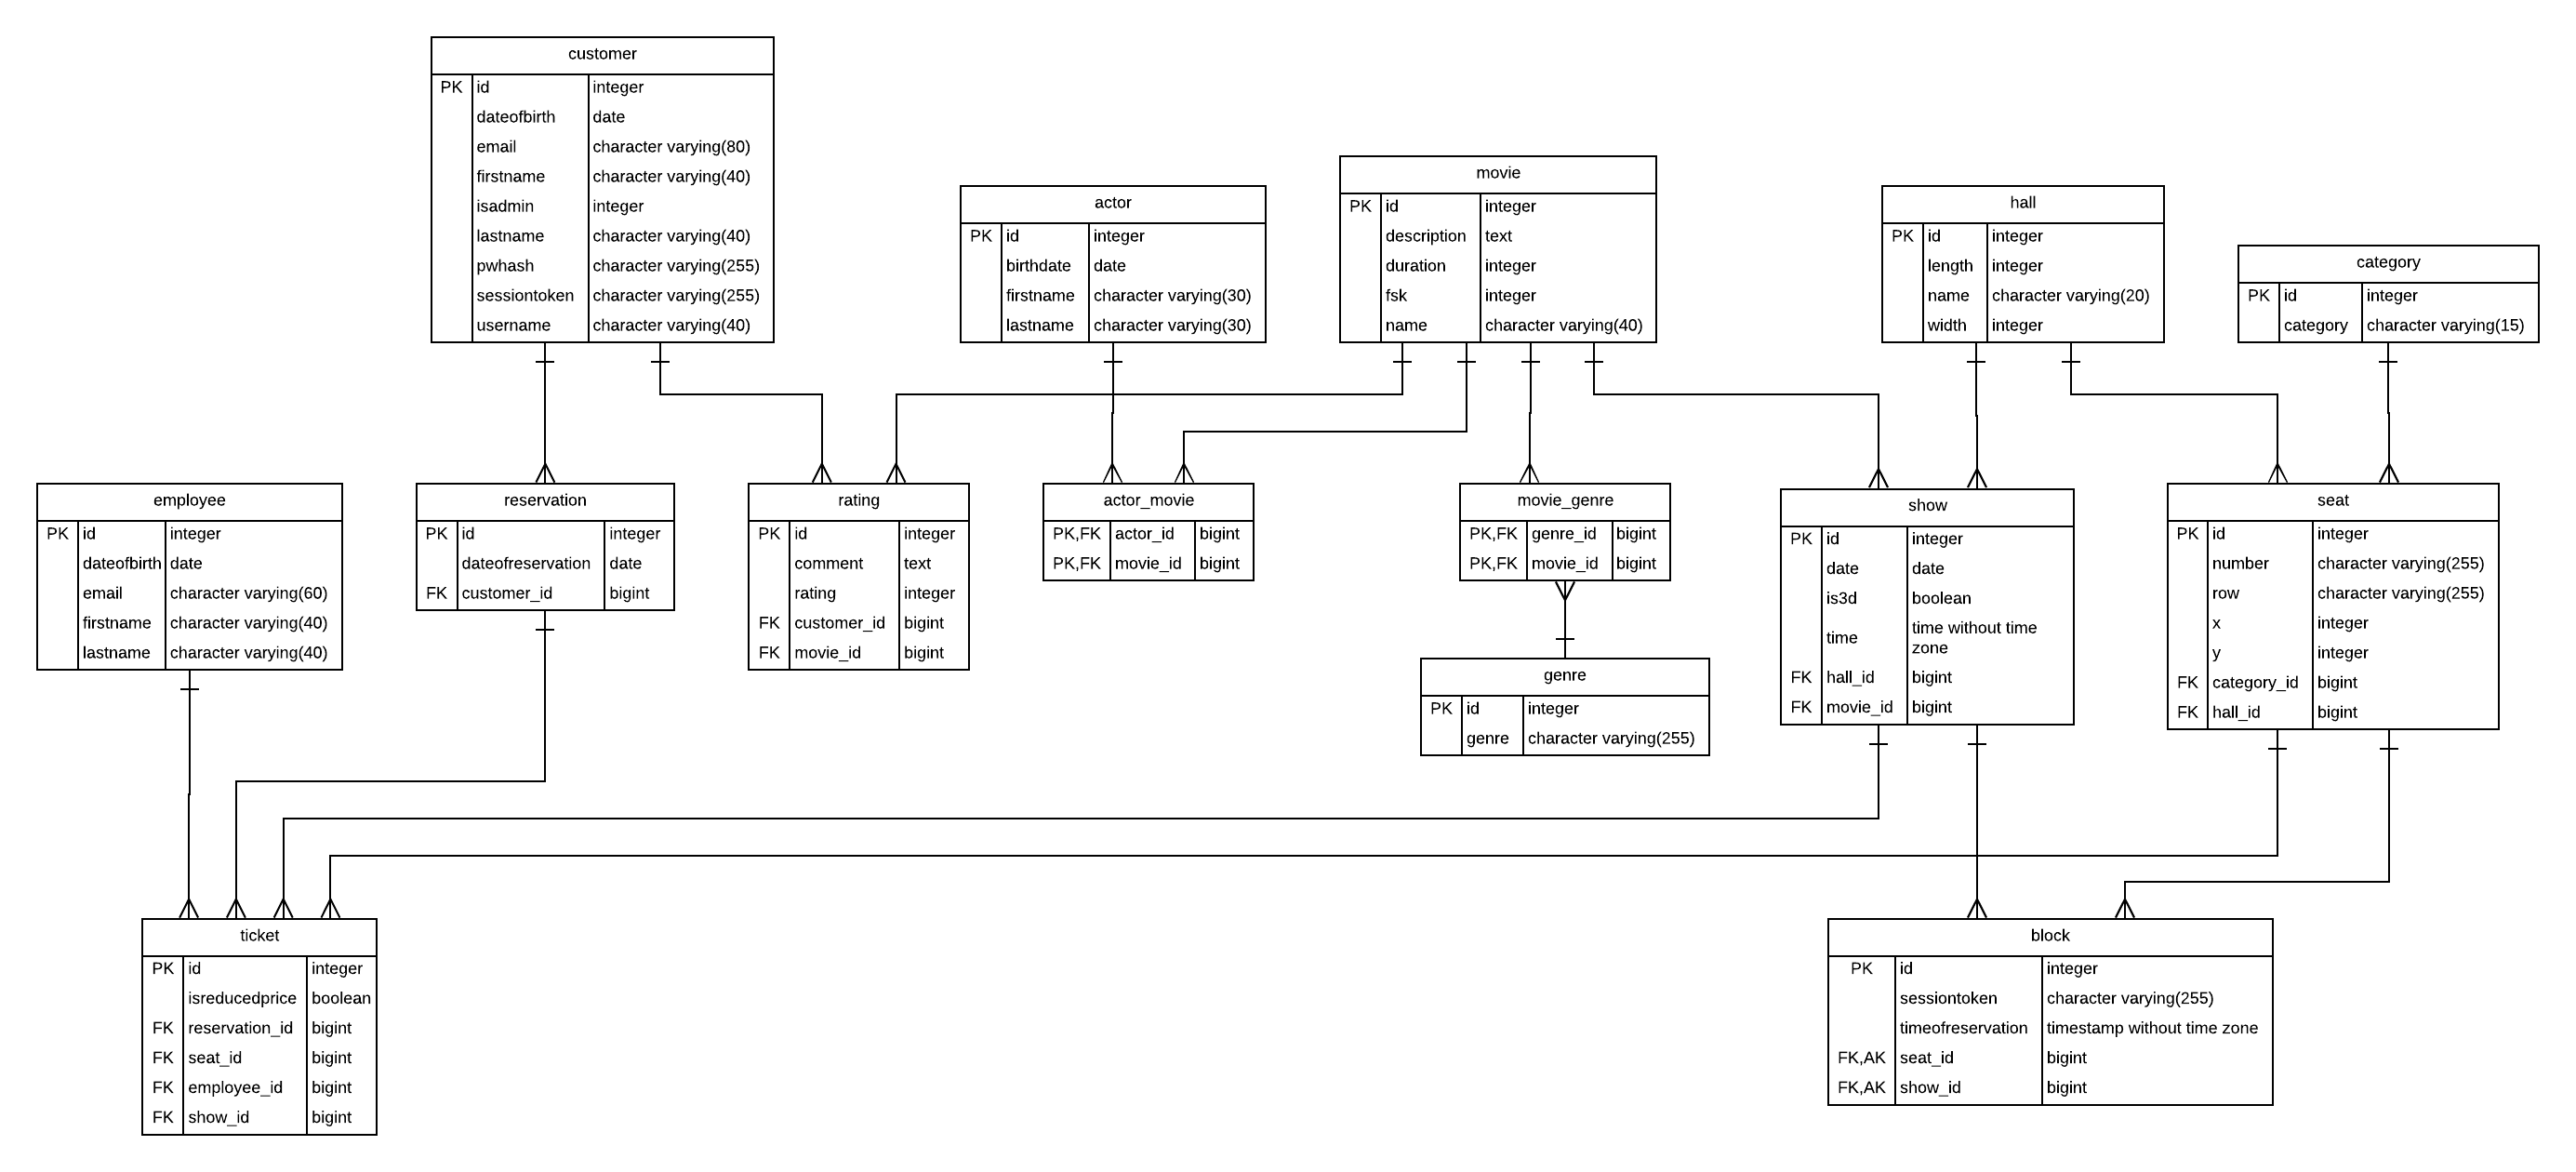
\includegraphics[keepaspectratio, width=1.0\textwidth, height=1.0\textheight]{img/ER-Modell}
	\captionsetup{format=hang}
	\caption{\acs{ER-Modell} der Datenbank}
	\small Quelle: eigene Darstellung mittels \url{https://www.lucidchart.com/}
	\label{fig:Anhang_ER-Modell}
\end{sidewaysfigure}

\chapter{Quellcode}
\begin{minipage}{\linewidth}
	\begin{lstlisting}[style=lstJava]
	public static MovieTo createMovieTo ( Movie entity, boolean withShow )
	{
	if ( null != entity )
	{
	MovieTo movieTo = new MovieTo();
	movieTo.setId(entity.getId());
	movieTo.setDescription(entity.getDescription());
	movieTo.setFsk(entity.getFsk());
	movieTo.setDuration(entity.getDuration());
	movieTo.setName(entity.getName());
	movieTo.setGenres(createGenreTos(entity.getGenres()));
	movieTo.setRatings(createRatingTos(entity.getRatings()));
	if ( withShow )
	{
	movieTo.setShows(createShowTos(entity.getShows(), false));
	} // end withSow
	movieTo.setActors(createActorTos(entity.getActors()));
	return movieTo;
	}  // end if null
	return null;
	}
	\end{lstlisting}
	\captionof{lstlisting}{Erstellen eines Movie-\acs{DTO} aus einer Movie-Entität mit Hilfe des eigen erstellten EntityToToHelper}
	\label{lst:EntityToToHelper_movie}
\end{minipage}

\begin{minipage}{\linewidth}
	\begin{lstlisting}[style=lstJava]
	public static Movie createMovieEntity ( MovieTo transferObject, boolean withShow )
	{
		if ( null != transferObject )
		{
			Movie movie = new Movie();
			movie.setId(transferObject.getId());
			movie.setActors(createActorEntities(transferObject.getActors()));
			movie.setDescription(transferObject.getDescription());
			movie.setFsk(transferObject.getFsk());
			movie.setDuration(transferObject.getDuration());
			movie.setName(transferObject.getName());
			movie.setRatings(createRatingEntities(transferObject.getRatings()));
			if ( withShow )
			{
				movie.setShows(createShowEntities(transferObject.getShows(), false));
			}
			movie.setGenres(createGenreEntities(transferObject.getGenres()));
			return movie;
		}
		return null;
	}
	\end{lstlisting}
	\captionof{lstlisting}{Erstellen einer Movie-Entität aus einem Movie-\acs{DTO} mit Hilfe des eigen erstellten ToToEntityHelper}
	\label{lst:ToToEntityHelper_movie}
\end{minipage}

% ewerkl.tex
% !TEX root =  master.tex

\clearpage
\chapter*{Ehrenwörtliche Erklärung}

Wir versichern hiermit, dass wir die vorliegende Arbeit
 mit dem Thema: \textit{\DerTitelDerArbeit} selbstständig verfasst und keine anderen als die angegebenen Quellen und
Hilfsmittel benutzt haben. Wir versichern zudem,
dass die eingereichte elektronische Fassung mit der gedruckten Fassung übereinstimmt.

\vspace{2cm}
Ort, Datum

\vspace{5mm}
\authorSG
\hfill \authorRF
\hfill \authorGP

\vspace{5mm}
\hfill \authorRF
\hfill \authorNL
\hfill

\end{document}
